\subsection*{\Large Общая характеристика работы}
\fontsize{14pt}{15pt}\selectfont
	%Обзор, введение в тему, обозначение места данной работы в мировых исследованиях и т.п.
\textbf{Актуальность темы исследования} 

Глобальный транспорт газов дыхательной и кровеносной системами является одним из основных процессов, связанных с жизнедеятельностью организма человека. Значительные и/или длительные отклонения от нормальных значений концентраций кислорода и углекислого газа в крови могут приводить к существенным патологическим изменениям, вызывающим необратимые последствия: недостаток кислорода (гипоксия и ишемические явления), изменение кислотно-щелочного баланса крови (ацидоз или алкалоз) и др. В условиях изменяющейся внешней среды и внутреннего состояния организма действие его регуляторных систем направлено на поддержание гомеостаза. 

Многие типичные изменения рисунка дыхания, такие как периодические и кластерные рисунки, связаны с конкретными заболеваниями и очень хорошо описаны в медицинской литературе. Кроме того, существует другая причина изменения картины дыхания: респираторная дисфункция. В этом случае имеют место хронические или повторяющиеся изменения в характере дыхания, которым нельзя дать конкретный медицинский диагноз, приводящие к жалобам пациентов с совершенно различными симптомами, такими как беспокойство, головокружения, усталость и т.д. В настоящее время не существует золотого стандарта для диагностики таких изменений рисунков дыхания вне их клинического описания. Более того, большинство специалистов по численному моделированию дыхательной системы в своих работах не уделяют особого внимания такого рода патологиям. Также для эффективного решения практических задач необходимо учитывать индивидуальную специфику каждого пациента, при этом возникает дилемма "точность модели/экономичность вычислений". Наибольшая точность может быть получена с помощью совместного решения трехмерных уравнений Навье-Стокса и уравнений деформируемого твердого тела по геометрии легких на основе данных компьютерной томографии(CT). Однако, для решения такой задачи обычно требуется вычислительный кластер либо длительное ожидание получения результата. Поэтому разработка моделей, которые с одной стороны максимально персонифицированы, и с другой стороны могут быть запущены на обычных компьютерах, является достаточно актуальной. 

Примером применения моделей транспорта дыхательных газов в медицине в условиях изменяющейся внешней среды является искусственная вентиляция легких(ИВЛ). При проведении хирургических операций под анестезией параметры ИВЛ контролируется анестезиологом, который выполняет корректировку параметров по отклонению параметров жизнедеятельности пациента. При такой схеме существует риск пере растяжения легких либо схлопывания альвеолярных объемов. В последнее время появляется большое количество работ, связанных с численным исследованием различных режимов ИВЛ. Одним из сдерживающих факторов в этом направлении является отсутствие достаточного объема медицинских данным в открытом доступе. Для данного направления также характерна проблема "точность модели/экономичность вычислений".   

Еще одной важной практической областью является моделирование глобального транспорта дыхательных газов при физической нагрузке. Одним из наиболее эффективных способов повышения спортивного результата является оптимизация тренировочного процесса. При этом важно индивидуальное дозирование уровня нагрузки и периодов отдыха. Дозировка достигаемого тренировочного воздействия производится тренером обычно опосредованно, на основе задания определенных значений "ключевых" параметров нагрузки: вида применяемых упражнений, их интенсивности и продолжительности, числа повторений упражнения и т.д. При этом предполагается, что между параметрами задаваемой нагрузки и изменениями тренируемой функции существуют определенные зависимости, на основе которых и становится возможным опосредованное управление тренировочным эффектом. Математические модели реакции организма на физическую нагрузку, с помощью которых можно рассчитывать тренировочный эффект, либо очень упрощенны и позволяют воспроизводить результаты только определенных протоколов нагрузки и не имеют большой прогностической способности, либо наоборот сложны(учитывают большое количество реакции), но очень локальны (подробно описывают процессы в определенной области организма) и не позволяют рассчитывать глобальный эффект. Поэтому критерием применимости моделей на практики является учет основных лимитирующих систем организма, позволяющий воспроизводить реакцию на различные протоколы нагрузки. Другой важной проблемой этой области является возможность идентификации модели по стандартным физиологическим тестам без применения сложного измерительного оборудования. 

\textbf{Научная новизна:}
\begin{enumerate}
 \item 
Разработан вычислительный, совместный 0D-1D метод расчета альвеолярного газообмена, позволяющий учитывать индивидуальную структуру легких, отличающийся вычислительно-экономичным способом стыковки много-масштабных моделей.
 \item 
 Разработан численный метод определения аэробного и анаэробного порогов, позволяющий получать большую точность по сравнению с аналогами за счет одновременного использования несколько физиологических показателей нагрузочного тестирования и специальной процедуры обработки зашумленных данных
 \item
 Разработана модель глобального газообмена у спортсменов при физической нагрузке, включающая в себя модели основных лимитирующих физические возможности систем: дыхательной, кровеносной, мышечного метаболизма, регуляции дыхания и кровообращения, отличающаяся небольшим количеством параметров, которые могут быть идентифицированы по тестам с возрастающей нагрузкой
 \item
 Разработана методика идентификации параметров модели по данным натурных экспериментов~--тестов с возрастающей нагрузкой, отличающаяся от аналогов тем, что идентификация выполнена для более сложной по структуре модели с использованием специальной обработки зашумленных данных и алгоритма глобальной стохастической оптимизации  
  
\end{enumerate}

\textbf{Научная и практическая значимость:} 

Подход из алгоритма стыковки 0D и 1D моделей легких может быть использован в  других, отличных от рассмотренных в работе, моделях легких.

Разработанный программный комплекс позволяет определять оптимальные параметры искусственной вентиляции на основе персональных CT-данных легких, а также исследовать изменения рисунка дыхания и эффективности альвеолярного газообмена при наличии различных патологий. Программный комплекс может быть использован для исследования других типов патологий легких.

Метод расчета аэробного и анаэробного порогов, реализованный в виде программного комплекса, используется экспертами-физиологами для быстрой и эффективной обработки данных нагрузочного тестирования.

Составные части комплексной модели реакции организма на физическую нагрузку могут быть интегрированы с другими более подробными моделями (например с 1D моделью гемодинамики).

Вычислительная методика идентификации параметров мышечного метаболизма по результатам нагрузочного тестирования может быть использована спортивными тренерами при оптимизации тренировочного процесса.

\textbf{Степень достоверности и апробация результатов.} 
Основные результаты работы были представлены на следующих научных конференциях и семинарах:

\noindent
\begin{itemize}
  
  \item 7-я (2015 г.), 8-я (2016 г.), 9-я (2017 г.) конференции по математическим моделям и численным методам в биоматематике (ИВМ РАН, г. Москва, Россия); 
  
  \item конференция "Экспериментальная и компьютерная биомедицина" (УрФУ, г.Екатеринбург, 10-12 апреля 2016)
  
  \item 57-я (2014), 58-я (2015) научные конференции МФТИ "Современные проблемы фундаментальных и прикладных наук" (г. Долгопрудный, Московская область, Россия)
  
  \item 3-я (2015), 4-я (2016), 5-я (2017) научно-практическая конференция "Инновационные технологии в подготовке спортсменов" (Центр спортивных технологий Москомспорта, г. Москва)
  
  \item семинары "Математические методы и модели в задачах спорта" (Центр спортивных технологий Москомспорта, г. Москва, Россия, 24 сентября 2015, 14 июня 2016 )
\end{itemize}

Основные результаты по теме диссертации опубликованы в 8 статьях и сборниках трудов конференций~\cite{GolovComp2017, GolovCmodel2017, GolovIt2017,GolovSp2015,GolovSp2016,TimmeSp2016,GolovEkb2016,Simakov2015}, из которых 2 изданы в журналах, рекомендованных ВАК \cite{GolovIt2017, GolovCmodel2017}, и 2 присутствуют в международной базе цитирования Web of Science \cite{GolovComp2017, GolovCmodel2017}.

Программный комплекс по определению аэробного и анаэробного порогов в настоящее время внедрен и используется специалистами ЦСТиСК Москомспорта.

Поданы заявки на регистрацию программ ЭВМ:
\begin{itemize}
    \item "Программа расчета глобального транспорта газов в организме человека"
    \item "Программа расчета аэробного и анаэробного порогов спортсменов по данным нагрузочного тестирования"
\end{itemize}
 
%\newpage
\subsection*{\Large Содержание работы}

\textbf{Объем и структура работы.} Диссертация состоит из~введения, четырех глав, заключения и~четырёх приложений. Полный объем диссертации составляет 145 страницу с~67~рисунками и~20~таблицами. Список литературы содержит 137~наименований.

Во \underline{\textbf{введении}} обосновывается актуальность исследований, проводимых в рамках данной диссертационной работы,  формулируется цель, ставятся задачи работы, сформулированы теоретическая и практическая значимость представляемой работы, описаны методы исследования, обоснована достоверность полученных результатов 

\subsection*{Первая глава}

В первой части приводится краткий обзор и анализ современных моделей дыхательной и сердечно-сосудистых систем, рассматривается применимость подходов для различных практических задач. Описываются методы для совместного расчета дыхательной и кровеносной систем при моделировании глобального транспорта веществ. Отдельное внимание уделяется связыванию кислорода и углекислого газа в крови, а также регуляции минутной вентиляции легких, сердечного выброса и перераспределения кровотока между органами для поддержания гомеостаза. Также описаны подходы и текущие сложности при моделировании мышечного метаболизма. 
\subsection*{Вторая глава}

Вторая глава посвящена моделям дыхательной системы. В \underline{\textbf{первом разделе}} описана совместная OD-1D модель. Для легких была выполнена декомпозиция структуры на проводящую зону (первые 4е поколения) и альвеолярные компоненты (8 компонент), каждая из которых осредняет альвеолы, альвеолярные ходы и бронхиолы. Параметры(топология, длина и диаметры бронхиальных трубок) 1D сетевой структуры легких были получены из 3D структуры трахейно-бронхиального дерева, которая была построена на основе анонимизированных данных компьютерной томографии легких. 
\begin{figure}[!ht]
	\centering
	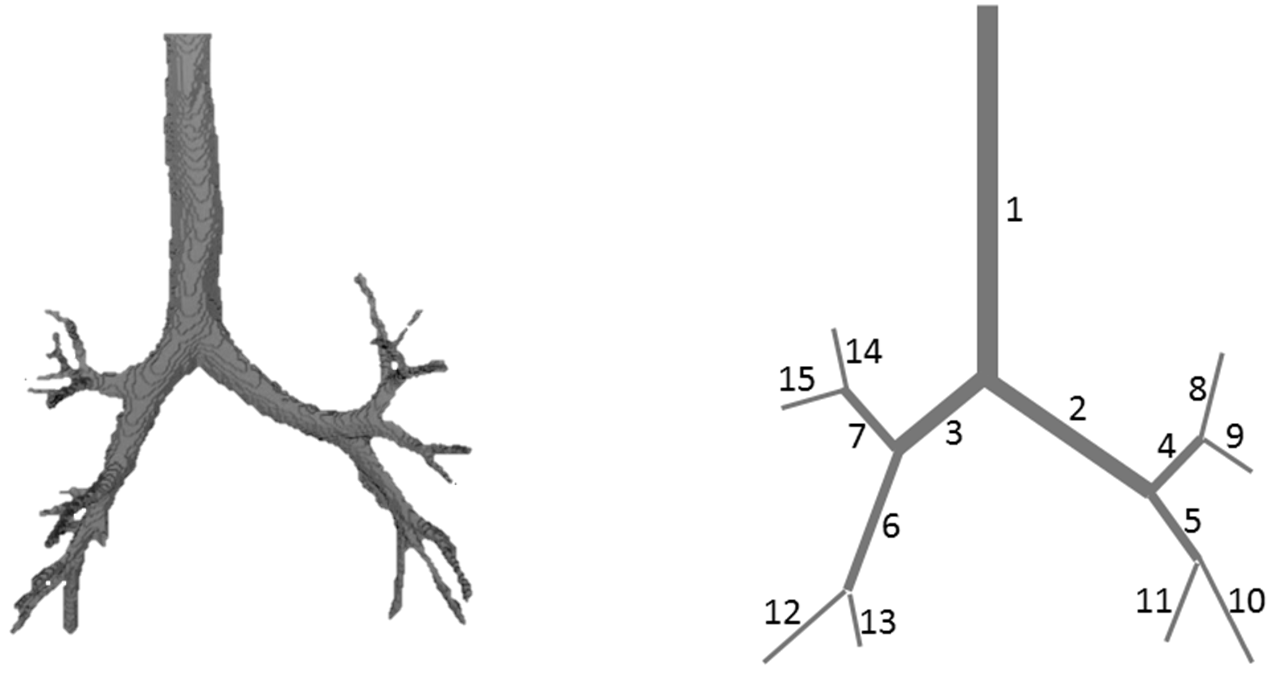
\includegraphics[scale=0.4]{ct.png}
	\caption{3D сегментация индивидуальных CT-данных трахейно-бронхиальной трубки и 1D сетевая структура на основе 3D сегментации} 
	\label{s2vechart}
\end{figure}
Поток воздуха в верхних дыхательных путях описывается с помощью уравнения сохранения массы и импульса в каждой отдельной трубке:
\begin{equation} 
\frac{\partial S_{k} }{\partial t} +\frac{\partial \left(S_{k} u_{k} \right)}{\partial x} =0 \notag
\end{equation} 
\begin{equation} 
\frac{\partial u_{k} }{\partial t} +\frac{\partial }{\partial x} \left(\frac{u_{k}^{2} }{2} +\frac{p_{k} \left(S_{k} \right)}{\rho } \right)=0 \notag  
\end{equation} 
где $t$ ~--время; $x$ ~--координата вдоль трубки; $k$ ~--индекс бронхиальной трубки; $\rho $ ~--плотность воздуха в бронхиальных трубках (принималась за константу); $S_{k} $ ~--площадь поперечного сечения трубки; $u_{k} \left(t,x\right)$ ~--линейная скорость потока воздуха, осредненная по площади поперечного сечения $S_{k} \left(t,x\right)$; $p_{k} \left(S_{k} \right)$ ~--плотность газа в бронхиальных трубках. 

Данная система дополняется "уравнением состояния":
\begin{equation} 
p_{k} \left(S_{k} \right)=\rho _{w} c_{0k}^{2} \left(\frac{S_{k} }{S_{0k} } -1\right)\notag  
\end{equation} 
где $\rho _{w} $ ~-- плотность материала бронхиальных трубок; $S_{0k} $ ~-- площадь поперечного сечения бронхиальной трубки в состоянии равновесия; $c_{0k} $ ~-- скорость распространения малых возмущений в материале стенок бронхиальных трубок

Граничное условие в области входа потока газа в носоглотку: 
\begin{equation}
p_{1} \left(S_{1} \left(t,0\right)\right)=p_{atm} =const. \notag 
\end{equation} 
Граничные условия в точке стыковки бронхиальных трубок определяются на основе закона сохранения массы и уравнения Бернулли:  
\begin{equation} 
S_{k_{1}^{n} } \left(t,L_{k_{1}^{n} } \right)u_{k_{1}^{n} } \left(t,L_{k_{1}^{n} } \right)=S_{k_{2}^{n} } \left(t,0\right)u_{k_{2}^{n} } \left(t,0\right)+S_{k_{3}^{n} } \left(t,0\right)u_{k_{3}^{n} } \left(t,0\right)\notag
\end{equation} 
\begin{equation} 
\frac{p_{k_{i} } \left(S_{k_{i} } \left(t,\tilde{x}_{k_{i} } \right)\right)}{\rho } +\frac{u_{k_{i} }^{2} \left(t,\tilde{x}_{k_{i} } \right)}{2} =I_{m} \left(t\right),\; i=1\div 3\notag 
\end{equation} 
где $\tilde{x}_{k} =L_{k} $~-- для входящих бронхиальных трубок; $\tilde{x}_{k} =0$ ~--для исходящих бронхиальных трубок, $L_{k} $ ~--длина бронхиальной трубки, $I_{n} \left(t\right)$ ~--инвариант потока.


Движение воздуха в переходной зоне описывается интегральной моделью для каждого альвеолярного объема:
\begin{equation} 
\frac{128\eta }{9\pi ^{2} V_{a}^{k} } \frac{dV_{a}^{k} }{dt} +E_{a}^{k} \left(V_{a}^{k} -V_{0a}^{k} \right)=p_{a}^{k} -p_{pl} \left(t\right) \notag
\end{equation} 
\begin{equation} 
V_{0a}^{k} = \frac{d_{k}^{2}}{\sum_{j=8}^{15} d^{2}_{j}}V_{0}^{tot} \notag
\end{equation}
где $k$ ~-- индекс альвеолярного компонента (соответствует индексу связанной терминальной бронхиальной трубкой), $V_{a}^{k} $ ~-- объем альвеолярного компонента; $V_{0a}^{k} $ ~-- объем альвеолярного компонента в не напряженном состоянии; $E_{a}^{k} $ ~--эффективная эластичность; $p_{a}^{k} $ ~--давление внутри альвеолярного компонента; $p_{pl} \left(t\right)$ ~--плевральное давление со стороны дыхательной мускулатуры, которое определяется из параметров дыхания; $V_{0}^{tot} $ ~-- суммарный объем легких в не напряженном состоянии.

Граничные условия в области стыковки альвеолярных объемов и бронхиальных трубок основаны на уравнениях сохранения массы и равенства давлений:
\begin{equation} 
\frac{dV_{ak} }{dt} =S_{k} \left(t,L_{k} \right)u_{k} \left(t,L_{k} \right)\notag  
\end{equation} 
\begin{equation} 
p_{ak} =p_{k} \left(t,L_{k} \right)\notag 
\end{equation} 

Расчет переноса дыхательных газов выполняется после подсчета параметров потока, описанными выше алгоритмами. При этом значения площади поперечного сечения бронхиальных трубок, линейные скорости потока и объемы альвеолярных компонент на верхнем временном слое $\left(t=t_{n+1} \right)$ являются известными. 
Перенос $O_{2}$ и $CO_{2}$ в верхних дыхательных путях описывается конвективным уравнением: 
\begin{equation}\label{GrindEQ__19_}
\frac{\partial C_{k,m} }{\partial t} +u_{k} \frac{\partial C_{k,m} }{\partial x} =0\notag 
\end{equation} 
где $m$ ~-- индекс вещества; $C_{k,m} $ ~-- доля(концентрация) вещества $m$ в $k^{ой} $ бронхиальной трубке.

Граничные условия для концентраций  в области входа потока газа в носоглотку во время вдоха $\left(u_{1} \left(t,0\right)>0\right)$: 
\begin{equation} 
C_{1,O_{2} } \left(t,0\right)=C_{O_{2} }^{atm} , C_{1,CO_{2} } \left(t,0\right)=C_{CO_{2} }^{atm} \notag
\end{equation} 
в случае $u_{1} \left(t,0\right)<0$ (выдох) значения концентраций определяются из уравнения переноса.

Граничные условия в точках бифуркаций бронхиальных трубок определяются из закона сохранения массы:
\begin{equation} 
\begin{array}{l} {C_{k_{1}^{p} ,m} \left(t,L_{k_{1}^{p} } \right)S_{k_{1}^{p} } \left(t,L_{k_{1}^{p} } \right)u_{k_{1}^{p} } \left(t,L_{k_{1}^{p} } \right)=} \\ {\; \; \; \; \; \; \; \; \; \; \; \; \; \; \; \; \; \; \; \; \; \; \; \; =C_{k_{2}^{p} ,m} \left(t,0\right)S_{k_{2}^{p} } \left(t,0\right)u_{k_{2}^{p} } \left(t,0\right)+C_{k_{3}^{p} ,m} \left(t,0\right)S_{k_{3}^{p} } \left(t,0\right)u_{k_{3}^{p} } \left(t,0\right)} \end{array}.  \notag 
\end{equation} 

Если $u_{k_{j}^{p} } \left(t,\tilde{x}_{k_{j}^{p} } \right)>0$, то $C_{k_{j}^{p} ,m} $ определяется из уравнения переноса вдоль выходящей характеристики. Если $u_{k_{j}^{p} } \left(t,\tilde{x}_{k_{j}^{p} } \right)<0$, то $ C_{k_{j}^{p} ,m} \left(t,\tilde{x}_{k_{j}^{p} } \right)=C_{p,m}^{node}$ 

Уравнение концентраций в альвеолярных объемах:
\begin{equation}  
\frac{d\left(C_{a,m}^{k} V_{a}^{k} \right)}{dt} =C_{k,m} S_{k} \left(t,L_{k} \right)u_{k} \left(t,L_{k} \right)+D_{m} S_{a}^{k} \left(C_{m}^{b} -C_{a,m}^{k} \right)\notag  
\end{equation} 


Уравнение концентрации в кровеносной системе(однокомпонентная модель):
\begin{equation} 
\frac{dC_{m}^{b} }{dt} =\frac{Q_{m}^{b} }{V^{b} } +D_{m} \sum _{k}\frac{S_{a}^{k} }{V^{b} } \left(C_{a,m}^{k} -C_{m}^{b} \right)\notag  
\end{equation}
где $k$ ~-- набор индексов альвеолярных компонент (в данной работе $k=8,...,15$); $C_{a,m}^{k} $ ~-- концентрация $m^{го} $  вещества в $k^{м} $ альвеолярном компоненте; $D_{m} $ ~-- коэффициент диффузии $m^{го} $ вещества между альвеолярным компонентом и кровеносной системой; $C_{m}^{b} $  ~-- концентрация $m^{го} $ вещества в кровеносной системе; $Q_{m}^{b} $ ~-- сток или источник $m^{го} $ вещества, соответствующий физиологическим данным в организме; $V^{b} $ ~-- полный объем крови в организме человека; $S_{a}^{k} $ ~-- эффективная площадь поверхности альвеолярного компонента

Предполагается, что дыхательный поток в дыхательных путях имеет, в основном, ламинарный характер. Состав дыхательного газа в альвеолярном объеме однородный, а сам газ несжимаемый. Также предполагаем, что при поступлении в легкие из внешней среды газ мгновенно нагревается и далее его температура постоянна, при этом также происходит его мгновенное насыщение водяными парами. 

Для ряда практических задач не требуется очень детальное описание воздушных потоков в легких, а необходимо воспроизводить только общую интегральную динамику. Для данных задач использовалась усредненная модель: 
\begin{equation}\label{AlvEq}
R\frac{dV}{dt}+E(V-V_{0})=P_{g}\sin wt, \notag
\end{equation}
\noindent где \( R\)~--- сопротивление дыхательных путей, \( E\) --- эластичность легких, \( V_{0}\) ~--- объем резервуара в не напряженном состоянии, \( w\) ~--- частота дыхания, \( P_{g}\)~---плевральное давление, \( t\) ~--- время. 

Дифференциальное уравнение имеет аналитическое решение, состоящее из постоянной, синусоидальной и экспоненциально затухающей компонент:
\begin{equation}\label{V_analyt}
V\left(t\right)=V_{0}+\frac{P_{g}}{R\sqrt{\lambda^2+w^2}}\sin \left( wt-\arctg\frac{w}{\lambda} \right)+\frac{P_{g}w}{R\left(\lambda^2+w^2\right)}e^{-\lambda t}, \lambda=\frac{E}{R} \notag
\end{equation}

Эмпирическая модель регуляции дыхания:
\begin{equation}
V_{E}=V_{SS}+\left(V_{C}+V_{P}\right)\left(1-e^{-\frac{t}{\tau}}\right) \notag
\end{equation}
\begin{equation}
V_{C}=K_{cCO_{2}}\left(P_{cCO_{2}}-T_{cCO_{2}} \right), V_{C}\ge 0 \notag
\end{equation}
\begin{equation}
V_{P}=K_{pCO_{2}}\left(P_{pCO_{2}}-T_{pCO_{2}} \right)+\left(\frac{570}{P_{pO_{2}}-26.2}-8.05\right)F(P_{pCO_{2}}), V_{P}\ge 0, \notag
\end{equation}
\begin{equation}
F(P_{pCO_{2}})=\begin{cases}
\left(5-4N_{pCO_{2}}^4 \right)^{-1}, & N_{pCO_{2}}\le 1 \\
N_{pCO_{2}}^3, & N_{pCO_{2}}> 1 
\end{cases}, 
N_{pCO_{2}}=\frac{P_{pCO_{2}}}{P_{pCO_{2}}^0} \notag
\end{equation}
\begin{equation}
V_{E}=nV_{T} \notag
\end{equation}
\begin{equation} 
\begin{cases}
n=n_{0},\; V_{T}=\frac{\displaystyle V_{E}}{\displaystyle n_{0}}; & V_{E} \le V_{E,T}  \\
V_{T}=\alpha V_{E}^{\displaystyle \beta},\; n= \frac{\displaystyle V_{E}}{\displaystyle V_{T}}; & V_{E} > V_{E,T}
\end{cases}\notag
\end{equation}
где \( V_{E}\)~--- минутная вентиляция легких, 
\( V_{SS}\)~--- минутная вентиляция легких в норме, 
\( V_{C}\)~--- регуляторный вклад центральных хеморецепторов,
\( V_{P}\)~--- регуляторный вклад периферических хеморецепторов,
\( \tau\)~--- параметр времени установления нового значения вентиляции, \( P_{cCO_{2}}\)~--- парциальное давление $CO_{2}$ в отделе центральных хеморецепторов, 
\( T_{cCO_{2}}\)~--- условно нормальное значение парциального давления $CO_{2}$ в отделе центральных хеморецепторов, 
\( K_{cCO_{2}}\)~--- коэффициент пропорциональности, \( T_{pCO_{2}}\) ~--- условно нормальное значение парциального давления $CO_{2}$ в отделе периферических хеморецепторов, 
\( K_{pCO_{2}}\)~--- коэффициент пропорциональности, 
\( P_{pO_{2}}, P_{pCO_{2}}\)~--- значения парциальных давлений $O_{2}$ и $CO_{2}$ в отделе периферических хеморецепторов,
\( P_{pCO_{2}}^0\)~--- референтное значение парциального давления $CO_{2}$ в отделе периферических хеморецепторов в норме, \( n\)  ~---  количество дыхательных циклов в минуту, \( V_{T}\)~--- дыхательный объем.

Во \underline{\textbf{втором разделе}} обсуждается численная реализация модели.
Алгоритм расчета на каждом шаге по времени разделяется на два этапа.  На первом этапе решаются уравнений баланса массы и импульса во внутренних узлах расчетной сетки для каждой бронхиальной трубки. Используется явная двухшаговая гибридная схема, соответствующая наиболее точной монотонной схеме первого порядка и наименее осциллирующей схеме второго порядка точности. На втором этапе с помощью метода Ньютона решается система нелинейных алгебраических уравнений на входах, выходах, точках бифуркаций для каждой бронхиальной трубки в граничных узлах расчетной сетки.

Исходная система уравнений баланса массы и импульса приведена к характеристическому виду
\begin{equation}
w_{ki} \cdot \left(\frac{dV_{k} }{dt} \right)_{i} =w_{ki} \cdot \left(\frac{\partial V_{k} }{\partial t} +\lambda _{ki} \frac{\partial V_{k} }{\partial x} \right)=0, i=1,2 
\end{equation}

Собственные значения  $\lambda_{ki}$ могут быть вычислены как:
\begin{equation} 
\lambda _{ki} =u_{k} +\left(-1\right)^{i} \sqrt{\frac{S_{k} }{\rho } \frac{\partial p_{k} }{\partial S_{k} } } =u_{k} +\left(-1\right)^{i} c_{0k} \sqrt{\frac{S_{k} }{S_{0k} } } ,\; i=1,2,  
\end{equation} 
В качестве левых собственных векторов можно выбрать:
\begin{equation} 
w_{ki} =\left(\begin{array}{c} {\sqrt{\frac{1}{\rho } \frac{\partial p_{k} }{\partial S_{k} } } } \\ {\left(-1\right)^{i} \sqrt{S_{k} } } \end{array}\right)=\left(\begin{array}{c} {\frac{c_{0k} }{\sqrt{S_{0k} } } } \\ {\left(-1\right)^{i} \sqrt{S_{k} } } \end{array}\right), i=1,2.  
\end{equation}

Для корректной постановки граничной условий произведена дискретизация условий совместности к виду
\begin{equation} 
u_{p}^{n+1} =\alpha _{p}^{n+1} S_{p}^{n+1} +\beta _{p}^{n+1} ,\; p=0,J.  
\end{equation} 

Коэффициенты $\alpha_k$ и $\beta_k$ зависят от вида дискретизации. 

Для дискретизации первого порядка $\alpha_k$ и  $\beta_k$:
\begin{equation}
\alpha _{p}^{n+1} =\frac{\left(-1\right)^{i+1} c_{0} }{\sqrt{S_{p}^{n} S_{0} } } 
\end{equation} 
\begin{equation} 
\beta _{p}^{n+1} =\frac{u_{p}^{n} +\left(-1\right)^{i} \sigma _{p}^{n} u_{q}^{n+1} -\alpha _{p}^{n+1} \left(S_{p}^{n} +\left(-1\right)^{i} \sigma _{p}^{n} S_{q}^{n+1} \right)}{1+\left(-1\right)^{i} \sigma _{p}^{n} } , \sigma _{p}^{n} =\frac{\tau _{n+1} }{h} \left(\lambda _{i} \right)_{p}^{n}  \notag
\end{equation} 

Для дискретизации второго порядка $\alpha_k$ и  $\beta_k$:
\begin{equation}
 \alpha _{p}^{n+1} =\frac{\left(-1\right)^{i+1} c_{0} }{\sqrt{S_{p}^{n} S_{0} } } ,
\end{equation} 
\begin{equation} 
\beta _{p}^{n+1} =\frac{u_{p}^{n} +\left(-1\right)^{i} \sigma _{p}^{n} \left(2u_{q}^{n+1}-0.5u_{z}^{n+1}\right) -\alpha _{p}^{n} \left(S_{p}^{n} +\left(-1\right)^{i} \sigma _{p}^{n} \left(2S_{q}^{n+1}-0.5S_{z}^{n+1}\right) \right)}{1+\left(-1\right)^{i}1.5\sigma _{p}^{n} } \end{equation} 

В точках стыковки терминальных трубок с альвеолярными компонентами используется неявная схемы Адамса второго порядка:
\begin{equation}
V_{a}^{n+1} =V_{a}^{n} +0.5\tau\left(S_{J}^{n+1} u_{J}^{n+1}+S_{J}^{n} u_{J}^{n}\right) .  
\end{equation} 
После дискретизации исходная система в точках стыковки сводится к полиномиальному уравнению 4й степени:
\begin{equation} 
\begin{array}
     \frac{128\eta }{9\pi ^{2} \left[V_{a}^{n} +0.5\tau\left(S_{J}^{n+1} u_{J}^{n+1}+S_{J}^{n} u_{J}^{n}\right) \right]} S_{J}^{n+1} u_{J}^{n+1} +\\+E_{a} \left[V_{a}^{n} +0.5\tau\left(S_{J}^{n+1} u_{J}^{n+1}+S_{J}^{n} u_{J}^{n}\right) -V_{0a} \right]=\rho c_{0}^{2} \left(\frac{S_{J}^{n+1} }{S_{0} } -1\right)-p_{pl}^{n+1} 
\end{array}
\end{equation} 
Численное исследование данного уравнения при физиологически адекватных значениях коэффициентов показало, что существует единственное корректное вещественное решение.  Данный алгоритм хорошо сходится для используемых при расчетах шагов по времени, которые ограничены условием устойчивости численной 1D схемы и являются достаточно малыми относительно характерных времен дыхательных циклов $\left(\tau \approx 10^{-4} s\right)$.

Численный алгоритм переноса дыхательных газов разделяется на отдельный расчет внутренних узлов расчетной сетки бронхиальных трубок с помощью схемы с разностью против потоков и граничных точек в областях бифуркаций бронхиальных трубок, входе в носоглотку и точках стыковки терминальных бронхиальных трубок и альвеолярных объемов, которые в случае необходимости дополняются выражением неявной дискретизацией, полученной для необходимого терминального узла (вход или выход в бронхиальную трубку), если поток газа в этом узле направлен за пределы рассматриваемой бронхиальной трубки.

В \underline{\textbf{третьем разделе}} описывается архитектура программного комплекса.

Программный комплекс состоит из трех основных компонент: модуля препроцессинга, решателя и модуля постпроцессинга. Модули препроцессинга и решателя на языке C++ с использованием ООП парадигмы и дополнительных библиотек Boost, Eigen, Intel Threading Building Blocks(TBB). Для расчета 60 сек. нормального синусоидального дыхания на двух ядерном Intel Core i3-2100 3.10GHz, Windows 7-64, 16Gb RAM требовалось в среднем 15 секунд. После окончания работы решателя запускается модуль постпроцессинга, в котором считываются логи вычислительного эксперимента. На основе логов рассчитываются агрегированные характеристики, при необходимости выполняется визуализация. Данный модуль написан на языке Python с использованием библиотек Numpy, Pandas и Matplotlib.

\subsection*{Третья глава}

В третьей главе обсуждается модель кровеносной системы и мышечного метаболизма.
Во \underline{\textbf{втором разделе}} описана модель кровеносной системы, основанная на разделении системы на пять крупных отделов, соответствующих артериям тканей, головного мозга и легких, системным и легочным венам.
\begin{figure}[!ht]
\centering
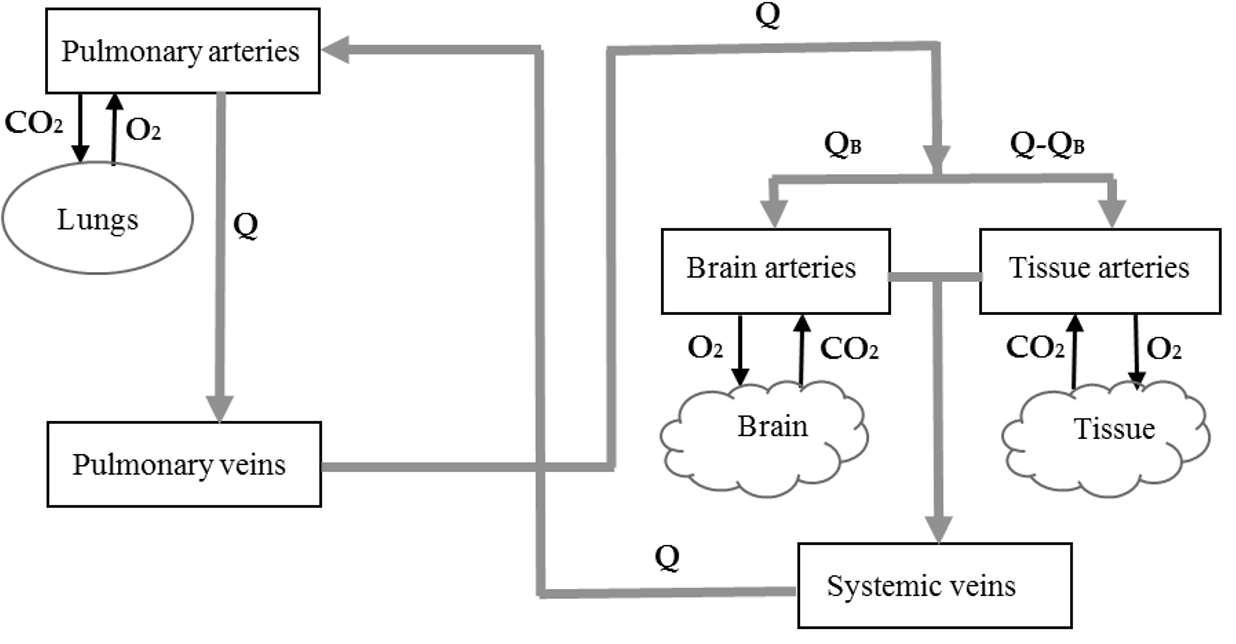
\includegraphics[width=0.7\textwidth]{System}
\caption{Общая схема модели кровеносной системы} \notag
\label{systemChart}
\end{figure}

Модель кровеносной системы и мышечного метаболизма сводится к решению 4х систем ОДУ:

1) Система ОДУ для концентрации лактата:
\begin{equation}
\frac{d\textbf{z}}{dt}=\textbf{A}\textbf{z}+\mathbf{\chi}_{LA}(\textbf{z})\notag
\end{equation}
\begin{equation}
\mathbf{\chi}_{LA}(\textbf{z})=\begin{pmatrix}
0 \\
0 \\
0 \\
0 \\
\displaystyle -u_{la}(z_{5}-C_{la,0})+\frac{W_{an}}{e_{la}V_{5}}
\end{pmatrix}\notag
\end{equation}
\begin{equation}
\mathbf{A}=\begin{pmatrix}
-\frac{Q_{0}}{V_{1}} & 0 & \frac{Q_{0}}{V_{1}} & 0 & 0 \\
\frac{Q_{0}}{V_{2}} & -\frac{Q_{0}}{V_{2}} & 0 & 0 & 0 \\
0 & 0 & -\frac{Q_{0}}{V_{3}} &  \frac{Q_{B}}{V_{3}} &  \frac{Q_{0}-Q_{B}}{V_{3}} \\
0 & \frac{Q_{B}}{V_{4}} & 0 & -\frac{Q_{B}}{V_{4}} & 0 \\
0 & \frac{Q_{0}-Q_{B}}{V_{5}} & 0 & 0 & -\frac{Q_{0}-Q_{B}}{V_{5}} \\
\end{pmatrix} \notag
\end{equation}
Где $\mathbf{z} = \{ C_{la,i} \}_{i \in [1,..,5]}$, $C_{la,i}$ концентрация лактата в $i$-м отделе кровеносной системы (1-легочные артерии, 2-легочные вены, 3-системные вены, 4-артерии головного мозга, 5-системные артерии), \( V_{i}\)~--- объем \(i\)-го отдела кровеносной системы, \( Q_{0}\) ~---минутный сердечный выброс, \( Q_{B}\) ~---минутный поток крови через артерии головного мозга, \(C_{la,0} \) ~--- концентрация лактата в покое, \(u_{la} \) ~--- скорость утилизации лактата в мышцах, миокарде, печени и кишечнике. \(u_{la} \) неизвестный параметр, который специфичен для каждого отдельного организма.

Энергия, необходимая для выполнения физического упражнения может быть получена аэробным и анаэробным путем: 
\begin{equation}\label{eq:W}
W=W_{a}+W_{an} \notag
\end{equation}
\begin{equation}\label{eq:Wa}
W_{a}=e_{a}\dot{V}_{O_{2},M} \notag
\end{equation}
\begin{equation}\label{eq:Wan}
W_{an}=e_{la}\dot{V}_{la}\notag
\end{equation}
\begin{equation} \label{eq:a_la_eqviv}
e_{la}=\frac{3M}{V_{blood}}e_{a} \notag
\end{equation}
Где \( W \) ~--- мощность упражнения \( W_{a} \) ~--- мощность, вырабатываемая за счет аэробных источников,  \( W_{an} \) ~--- мощность, вырабатываемая за счет анаэробных источников, \( \dot{V}_{O_{2},M} \) ~--- мышечный кислородный запрос упражнения, \(e_{a}\) ~--- энергетический эквивалент кислорода, \( \dot{V}_{la} \) ~--- скорость образования лактата, \(e_{la}\) ~--- энергетический эквивалент лактата,\( M \)  ~---масса тела, \(V_{blood}\) ~--- общий объем крови

Лактатный(анаэробный) порог ($W_{LT}$)~--- мощность упражнения, при которой вклад анаэробного метаболизма становится заметным. Данная зависимость определяется безразмерной функцией $\sigma$:
\begin{equation} \label{eq:sigma}
\sigma\left(W\right) = W_{a} / W = 1-\beta e^{\alpha(W-W_{LT})} \notag
\end{equation}
Где $\alpha > 0, 0 < \beta < 1$  ~---неизвестные параметры, который специфичны для каждого отдельного организма. Значение функции $\sigma\left(W\right)$ примерно равно 1 в случае $W < W_{LT}$ и уменьшается в случае $W > W_{LT}$. Значения параметров $\alpha$ и $\beta$ должны быть определены так, что $\sigma\left(W\right) > 0$ для физиологического интервала значений $W$.

2) Система ОДУ для значения $Hc_{i}=C_{HCO_{3}^{-},i}-C_{H^{+},i}, \mathbf{Hc} = \{ Hc_i \}_{i \in [1,..,5]}$:
\begin{equation}
\frac{d \textbf{Hc}}{dt}= \mathbf{A Hc} \notag
\end{equation}

3) Система ОДУ для $CO_{2}$:
\begin{equation}
\displaystyle \frac{d\textbf{y}}{dt}
=\mathbf{A}\mathbf{\xi}_{CO_{2}}(\textbf{y})+\mathbf{\chi}_{CO_{2}}(\textbf{y})\notag
\end{equation}
\begin{equation}
\mathbf{\xi_{CO_{2}}}(\textbf{y})_{i}=\frac{y_{i}^2+(K_{CO_{2}}-Hc_{i})y_{i}}{S_{CO_{2}}(y_{i})K_{CO_{2}}}, S_{CO_{2}}(y_{i})=\frac{K_{CO_{2}}-Hc_{i}+2y_{i}}{K_{CO_{2}}}\notag
\end{equation}
\begin{equation}
\mathbf{\chi}_{CO_{2}}(\mathbf{y})=\begin{pmatrix}
\displaystyle \frac{D_{CO_{2}}S}{V_{1}S_{CO_{2}}(y_{1})}\left(P_{CO_{2},alv}-\frac{y_{1}^2-Hc_{1}y_{1}}{K_{CO_{2}} \sigma_{CO_{2}}} \right) \\
0 \\
0 \\
\displaystyle \frac{\dot{V}_{CO_{2},B}}{V_{4}S_{CO_{2}}(y}_{4}) \\
\displaystyle \frac{1}{V_{5}S_{CO_{2}}(y_{5})}\left(\dot{V}_{CO_{2},T}+\dot{V}_{O_{2},M}RQ+\kappa_{CO_{2}}\left(z_{5}-C_{la,0}\right) \right)
\end{pmatrix} \notag
\end{equation}
Где $\mathbf{y} = \{ C_{HCO_{3}^{-}},i \}_{i \in [1,..,5]}$ ~--- концентрация $HCO_{3}^{-}$ в $i$-м отделе кровеносной системы, \( \sigma_{CO_{2}} \) ~--- коэффициент растворимости \( CO_{2}\) в крови, \( \dot{V}_{CO_{2},B}\) ~---выделение \( CO_{2}\) мозгом, \( \dot{V}_{CO_{2},T}\) ~---выделение \( CO_{2}\) тканями, \( P_{CO_{2},alv} \) ~--- парциальное давление \( CO_{2}\) в альвеолярном объеме, \(\kappa_{CO_{2}} \) ~--- коэффициент неметаболического образования \(CO_{2} \), $\displaystyle RQ=\frac{\dot{V}_{CO_{2},T}}{\dot{V}_{O_{2},T}}$  ~---дыхательный коэффициент в покое, $\dot{V}_{O_{2},M}$ ~--- объем кислорода, потребляемый мыщцами при физической работе, $K_{CO_{2}}=\frac{k_{CO_{2}}^{-}}{k_{CO_{2}}^{+}}$, \( k_{CO_{2}}^{+}\)~--- скорость прямой реакции гидратации молекул \( CO_{2}\), \( k_{CO_{2}}^{-}\)~--- скорость обратной реакции гидратации молекул \( CO_{2}\).

4) Система ОДУ для $O_{2}$:
\begin{equation}
\displaystyle \frac{d\textbf{x}}{dt}
=\mathbf{A} \mathbf{\xi}_{O_{2}}(\textbf{x})+\mathbf{\chi}_{O_{2}}(\textbf{x}), S_{O_{2}}(\textbf{x}_{i})=1+\frac{m^2K_{O_{2}}T_{Hb}x_{i}^{m-1}}{\left( K_{O_{2}}+x_{i}^m\right)^2}\notag
\end{equation}
\begin{equation}
\mathbf{\xi}_{O_{2}}(x)_{i}=\frac{\displaystyle x_{i}+\frac{m T_{Hb}x_{i}^{m}}{ K_{O_{2}}+x_{i}^m}}{S_{O_{2}}(x_{i})}\notag
\end{equation}
\begin{equation}
\mathbf{\chi}_{O_{2}}(\textbf{x})=\begin{pmatrix}
\displaystyle \frac{D_{O_{2}}S}{V_{1}S_{O_{2}}(x_{1})}\left(P_{O_{2},alv}-\frac{x_{1}}{\sigma_{O_{2}}} \right) \\
0 \\
0 \\
\displaystyle -\frac{\dot{V}_{O_{2},B}}{V_{4}S_{O_{2}}(x}_{4)} \\
\displaystyle -\frac{1}{V_{5}S_{O_{2}}(x_{5})}\left(\dot{V}_{O_{2},T}+\dot{V}_{O_{2},M}\right)
\end{pmatrix}\notag
\end{equation}
Где $\mathbf{x}=\{ C_{O_{2},f,i} \}_{i \in [1,..,5]}$, $C_{O_2,f}$ концентрация $O_2$, растворенного в плазме в $i$-м отделе кровеносной системы, \( \sigma_{O_{2}} \) ~--- коэффициент растворимости \( O_{2}\) в крови, \( \dot{V}_{O_{2},B}\) ~---потребление \( O_{2}\) мозгом, \( \dot{V}_{O_{2},T}\) ~---потребление \( O_{2}\) тканями, \( P_{O_{2},alv} \) ~--- парциальное давление \( O_{2}\) в альвеолярном объема, $T_{Hb}$ ~---суммарная концентрация гемоглобина в крови, $K_{O_{2}}=\frac{k_{O_{2}}^{-}}{k_{O_{2}}^{+}}$, \( k_{O_{2}}^{+}\)~--- скорость прямой реакции образования оксигемоглобина, \( k_{O_{2}}^{-}\)~--- скорость обратной реакции образования оксигемоглобина

Во \underline{\textbf{втором разделе}} выполнено аналитическое исследование модели кровеносной системы и мышечного метаболизма. Были определены точки равновесия, тип устойчивости и физиологически допустимые соотношения между параметрами.

В \underline{\textbf{третьем разделе}} описаны численные методы.
Модель кровеносной системы и мышечного метаболизма сводится к решению четырех задач Коши для систем ОДУ вида:

\begin{equation} \label{eq:Koshi}
\frac{d\mathbf{x}(t)}{dt}=\mathbf{f}(t,\mathbf{x}(t)), \, \mathbf{x}(0)=\mathbf{x_0}\notag
\end{equation}

Коэффициент жесткости системы:
\begin{equation}
    \zeta = \frac{\max \limits_{Re \, \lambda_k < 0} \mid Re \, \lambda_k \mid}{\min \limits_{Re \, \lambda_k < 0} \mid Re \, \lambda_k \mid}\notag
\end{equation}

Где $\lambda_k$~---собственные значения матрицы Якоби $\displaystyle \mathbf{f}_\mathbf{x} = \left\{ \frac{\partial \mathbf{f}}{\partial \mathbf{x}} \right\}$

Значения $\lambda_k$ были численно определены при физиологическом диапазоне входных параметров. Эксперименты показали, что для системы №1: \(\zeta \sim 10\), для системы №2: \(\zeta \sim 10^{4}\), для системы №3: \(\zeta \sim 10\), для системы №4: \(\zeta \sim 10^{5}\). Таким образом система уравнений для кровеносной системы является жесткой и необходимо применение специальных численных методов. Для решения жестких систем ОДУ использовался неявный одношаговый A,L - устойчивый метод третьего порядка аппроксимации из семейства схем Обрешкова. 

Для совместного расчета уравнений дыхательной системы, кровеносной и мышечной систем на каждом временном шаге до достижения критерия сходимости выполнялась итерационная процедура, включающая блоки расчета мышечного метаболизма, системных величин (дыхательный объем, объем легких, сердечный выброс и т.д.), баланса газов ($O_2, CO_2$) и лактата в крови:

\begin{enumerate}
	
	\item {\it Мышечный метаболизм.}

\begin{enumerate}
	
	\item \label{it:iter_start} Расчет доли аэробного энергопотребления ($\sigma$), уровеня потребления кислорода ($\dot{V}_{O_{2},M}$). 
	
	\item Расчет уровня производства лактата ($\dot{V}_{la}$) в следствии анаэробного метаболизма.
	
\end{enumerate}	

	\item {\it Системные величины.}

\begin{enumerate}
		
	\item Расчет дыхательного объема $V_{T}$ и количества дыхательных циклов в минуту. 
	
	\item Расчет минутного  $Q_{0}$ и минутного потока крови в артерии головного мозга. 
	
	\item Расчет объема легких $V(t)$, текущих альвеолярных концентрации $O_{2}$ и $CO_{2}$.   

\end{enumerate}

	\item {\it Баланс газов и лактата в крови.}

\begin{enumerate}	
	
	\item Определяются вектора начальных значений:
	\begin{equation*}
	\tilde{\mathbf{x}}^{n+1} = \mathbf{x}^{n}, \tilde{\mathbf{y}}^{n+1} = \mathbf{y}^{n}, \tilde{\mathbf{z}}^{n+1} = \mathbf{z}^{n}, \mathbf{\tilde{H}c}^{n+1} = \mathbf{Hc}^{n}, 
	\end{equation*}
	где $\tilde{\mathbf{x}}^{n+1}$, $\tilde{\mathbf{y}}^{n+1}$, $\tilde{\mathbf{z}}^{n+1}$, $\tilde{\mathbf{Hc}}^{n+1}$ текущие значения векторов концентраций соответствующих веществ в отделах кровеносной системы.
	
	\item Расчет значение $\tilde{\mathbf{z}}^{n+1}$, $\tilde{\mathbf{x}}^{n+1}$, $\mathbf{\widetilde{H}c}^{n+1}$.
	
	\item Расчет значения $\tilde{\mathbf{y}}^{n+1}$ с использованием значений $\tilde{\mathbf{x}}^{n+1}$, $\tilde{\mathbf{z}}^{n+1}$, $\mathbf{\widetilde{H}c}^{n+1}$.
	% Task~4. 

\end{enumerate}

	\item {\it Проверка критерия сходимости алгоритма.}
	
	 Критерий сходимости, при удовлетворении которого итерационная процедура останавливается:
	\begin{equation*}
	\delta \left( \tilde{\mathbf{x}}^{n+1}, \mathbf{x}^{n+1} \right) < \varepsilon, \delta \left( \tilde{\mathbf{y}}^{n+1}, \mathbf{y}^{n+1} \right) < \varepsilon, \delta \left( \tilde{\mathbf{z}}^{n+1}, \mathbf{z}^{n+1} \right) < \varepsilon, \delta \left( \mathbf{\tilde{H}c}^{n+1}, \mathbf{Hc}^{n+1} \right) < \varepsilon,
	\end{equation*}
	Где $\delta \left( \tilde{\mathbf{s}}^{n+1}, \mathbf{s}^{n+1} \right) = \displaystyle \frac{\|\tilde{\mathbf{s}}^{n+1} - \mathbf{s}^{n+1}\|}{\|\mathbf{s}^{n+1}\|}$, $\|\mathbf{s}\| = \max \limits_j \left| s_j \right|$; $\tilde{\mathbf{s}}^{n+1}$, $\mathbf{s}^{n+1}$, $\mathbf{s}$ вектора одинаковой размерности. 
	
	Иначе итерационная процедура продолжается с новыми значениями:
	\begin{equation*}
	{\mathbf{x}}^{n+1} = \tilde{\mathbf{x}}^{n+1}, \mathbf{y}^{n+1} = \tilde{\mathbf{y}}^{n+1}, \mathbf{z}^{n+1} = \tilde{\mathbf{z}}^{n+1}, \mathbf{Hc}^{n+1} = \mathbf{\tilde{H}c}^{n+1}.
	\end{equation*}

\end{enumerate}

Параметры модели мышечного метаболизма: \(e_{a}, u_{la}, \kappa_{CO_{2}}\), $\beta$, $\alpha$ могут сильно отличаться для каждого человека. При этом корректное определение значений данных параметров очень сильно влияет на точность результатов модели. Остальные значения параметров модели могут быть взяты, как средние по популяции, либо с использование алло-метрических показателей на основе роста и веса.  

Неизвестные параметры идентифицировались по результатам физиологических нагрузочных тестов, во время которых регистрируются показатели потребления \(O_{2}\), выделения \(СO_{2}\), минутной вентиляции легких \(V_{E}\), и концентрации лактата (LA). 
Оптимальные значения параметров мышечного метаболизма $e_{a}$, $u_{la}$, $\kappa_{CO_{2}}$, $\beta$, $\alpha$ определялись из минимизации функционала с помощью алгоритма дифференциальной эволюции ~--- стохастического алгоритма глобально оптимизации:
\begin{equation} \label{eq:functional}
\Phi = \sum \limits_{M \in \{O_2, CO_2, V_E, LA\}} \left( \frac{1}{N_M}\sum_{i=1}^{N_M} huber\left(\Delta_{M,i}\right) \right),
\end{equation}
\noindent Где
\begin{equation} \label{eq:huber}
huber(\Delta)=\begin{cases}
\frac{1}{2}\Delta^2,& |\Delta| \le \delta\\
\delta(|\Delta|-\frac{1}{2}\delta),& |\Delta| > \delta
\end{cases}, 
\Delta_{M,i}=\frac{x_{M,i}^{exp}-x_{M,i}^{num}}{x_{M,i}^{exp}}, \delta_M = 1.5\sqrt{\frac{1}{N_M}\sum_{i=1}^{N_M}\Delta_{M, i}^{2}},
\end{equation}
\noindent $M$~---индекс параметра (($O_{2}$)- объем потребления $O_{2}$, ($CO_2$)- объем выделения $CO_{2}$, ($LA$)- концентрация лактата в крови , ($V_E$)- минутная вентиляция легких ), $N_M$~--- количество экспериментальных измерений параметра $M$, $x_{M,i}^{exp}$ ~--- $i$-ое измерение значения параметра $M$, $x_{M,i}^{num}$ ~--- $i$-ое расчетное значение параметра $M$.

В модели мышечного метаболизма используется значение анаэробного порога(ПАНО). Корректность определения анаэробного порога во многом влияет на точность модели. Значение ПАНО определялось по показателям тестов с возрастающей нагрузкой на беговой дорожке.  В уравнение регрессии показателя ExсСО2, состоящей из 2-х частей, присутствует одна точка перегиба. Уравнения регрессии показателей VCO2, RER, VE состоят из 3-х кусочно-линейных участков и имеют две точки перегиба. Неизвестные параметры определяются из минимизация функционал среднеквадратичных ошибок. Для повышения устойчивости к выбросам используется робастная версия алгоритма. Для значения каждого параметра модели может быть выполнен расчет доверительного интервала (ДИ). Расчет ДИ выполняется с помощью модифицированного для временных серий метода бутстреппинга ~--- the moving block bootstrap. АэП и ПАНО определяются. как среднее значение ДИ по всем показателям газоанализа. 

В \underline{\textbf{четвертом разделе}} представлено описание архитектуры программных комплексов. Модель кровеносной системы и мышечного метаболизма реализована в виде программного комплекса с использованием абстрактной модели и архитектуры программного комплекса совместной 0D-1D модели. Для расчета 900 сек. нагрузочного теста на двух ядерном Intel Core i3-2100 3.10GHz, Windows 7-64, 16Gb RAM требовалось в среднем 10 секунд. Был добавлен дополнительный модуль оптимизации на языке Python.

Алгоритм определения анаэробного порога был реализован в виде отдельного программного комплекс на языках JavaScript и C\#. Данный комплекс был внедрен в ЦСТиСК Москомспорта. 

\subsection*{Четвертая глава}

В четвертой главе представлены результаты численных расчетов с использованием разработанных моделей.

Для описания транспорта газов в кровеносной системе используется модель, основанная на разделении системы на пять крупных отделов, соответствующих артериям тканей, головного мозга и легких, системным и легочным венам.


В \underline{\textbf{первом разделе}} выполнена проверка адекватности 0D-1D модели дыхательной системы. После подбора параметров в физиологических пределах, модель показала хорошее совпадение альвеолярного потока и альвеолярного давления в нормальных условиях с литературными данными.

Во \underline{\textbf{втором разделе}} с помощью численной модели дыхательной системы выполнено изучение зависимости альвеолярной концентрации $CO_{2} $ от частоты дыхательных циклов при проведении искусственной вентиляции легких(ИВЛ). Минимизация значения концентрации $CO_{2} $ рассматривалась как критерий эффективности функционирования легких. Выполнен поиск оптимальной чистоты(обеспечивающей наилучший газообмен) ИВЛ. Полученное значение(0.17 Hz) находится достаточно близко к экспериментально измеренной величине чистоты дыхания пациента в нормальном состоянии(0.23 Hz).

В \underline{\textbf{третьем разделе}} выполнено моделирование патологических рисунков дыхания: дыхание Биота и Чейна-Стокса. Величины альвеолярных концентраций $CO_{2} $ и $O_{2} $, полученные в результате численных расчетов показаны на рисунках . При нормальном дыхании альвеолярная концентрация $CO_{2} $ остается в пределах 4.8-5.9\%. При дыхании Биота и Чейна-Стокса данный интервал заметно изменяется.  При дыхании Биота альвеолярная концентрация $CO_{2} $ увеличивается до 8.4\%, наибольшее значение данного параметра достигается при дыхании Чейна-Стокса(8-10.4\%). При нормальном дыхании альвеолярная концентрация $O_{2} $ остается в пределах 13.9-15.1\%. Этот интервал имеет более широкие границы при дыхании Биота с нижним значением 10.7\%. Наибольшее уменьшение альвеолярной концентрации $O_{2} $ было получено для дыхания Чейна-Стокса (8-11\%).

Таким образом, в случае патологических типов дыхания: Биота и Чейна-Стокса наблюдается заметные изменения альвеолярных концентраций $CO_{2} $ и $O_{2} $ по сравнению с нормальным дыханием.

В \underline{\textbf{четвертом разделе}} выполнено моделирование легких, умеренных и тяжелых приступов астмы при помощи уменьшения площади поперечного сечения терминальных трубок трахейно-бронхиального дерева $S_{0} $, а также эффективного радиуса альвеолярных объемов $r_{ef} $ при помощи зависимости:
\begin{equation} \label{GrindEQ__43_} 
S_{0}^{\gamma } =\pi \left(r_{ef}^{\gamma } \right)^{2} =S_{0}^{norm} {\left(100-\gamma \right)\mathord{\left/ {\vphantom {\left(100-\gamma \right) 100}} \right. \kern-\nulldelimiterspace} 100} ,  
\end{equation} 
где $S_{0}^{\gamma } $, $r_{eff}^{\gamma } $ ~-- модифицированные значения площади поперечного сечения и эффективного радиуса во время приступа астмы;

Значения дыхательного объема и альвеолярной концентрации $O_{2} $ незначительно изменяются при легком приступе астмы ($0\% \le \gamma \le 20\% $), при этом, величина альвеолярной концентрации $CO_{2} $ остается стабильной. Незначительные изменения связаны с наличием резервов кардио-респираторной системы по доставке  $O_{2} $ и выведению  $CO_{2} $. Умеренные приступы астмы ($20\% \le \gamma \le 40\% $) характеризуются заметным уменьшением значения дыхательного объема и альвеолярной концентрации $O_{2} $, а также значительному нарастанию парциального давления $CO_{2} $, ацидоз продолжает прогрессировать. Случай тяжелого приступа астмы ($\gamma >40\% $) характеризуется дальнейшим резким изменением всех описанных выше параметров, которые выходят за физиологические пределы при $\gamma >50\% $. При таком воздействии кардио-респираторная система перестает справляться с поддержанием газообменом на нужном уровне, и без дополнительных воздействий система уже не приходит к состоянию равновесия. Таким образом, верхний предел тяжелого случая астмы, полученный при численном моделировании, находится при значении $\gamma =50\% $.

В \underline{\textbf{пятом разделе}} выполнено моделирование минутной вентиляции легких в условиях гиперкапнии. Для испытуемых изменяли состав вдыхаемого газа, увеличивая в нем содержание \(CO_{2}\) в интервале от 3\% до 7\%. Данный эксперимент отчасти воспроизводит тренировочные условия, целью которых является легальное повышение гемоглобина в крови у спортсменов уровня олимпийской сборной.

Достигнута высокая степень согласованности между результатами численного моделирования и лабораторных исследований. Для случая гипоксии наблюдались значительные отклонения на начальном этапе эксперимента. Однако, модель позволяет удовлетворительно (в пределах погрешности эксперимента) воспроизвести установившееся значение минутной вентиляции (через $10$~мин. после начала эксперимента) рис.~\ref{image9}.
\begin{figure}[!ht]
    \centering
	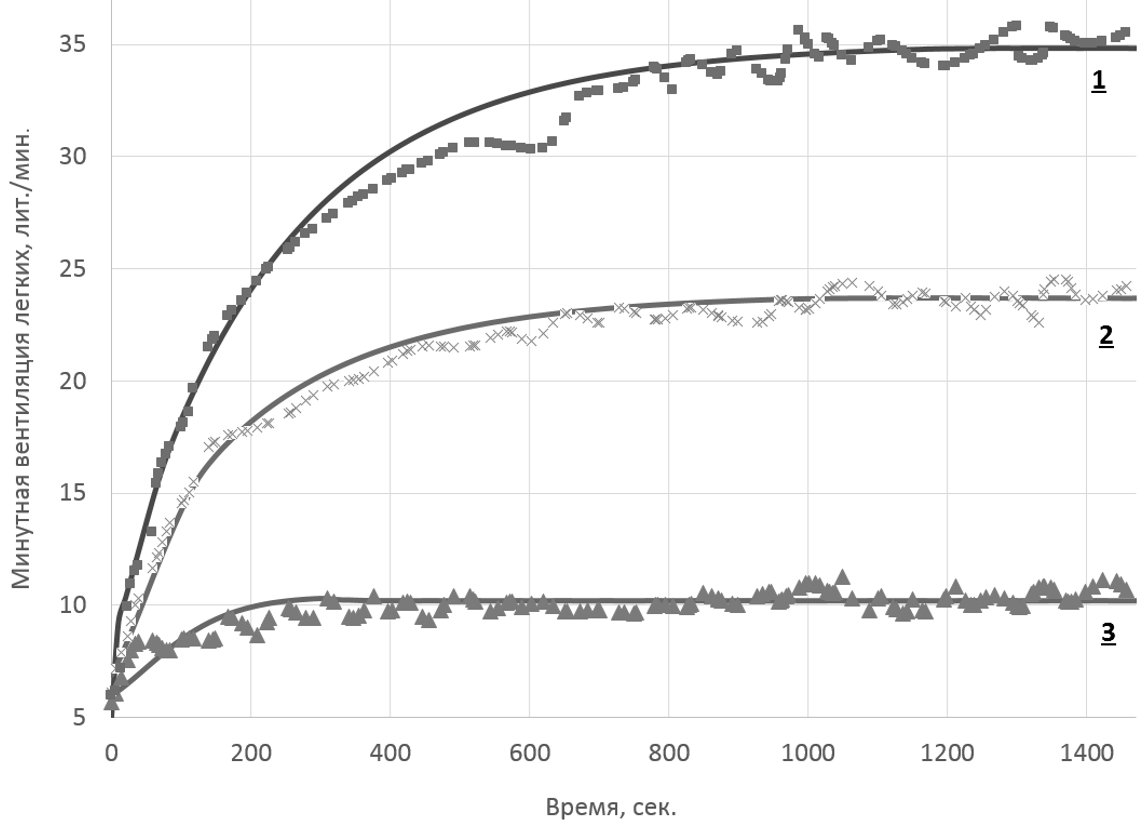
\includegraphics[scale=0.4]{hyper.png}
	\caption{Сравнение изменения минутной вентиляции легких в условиях гиперкапнии при лабораторных исследованиях и численном моделировании (данные расчетов обозначены сплошными линиями). 1 ~--- \(7\% \;CO_{2}\), 2 ~--- \(6\% \;CO_{2}\), 3 ~--- \(3\% \;CO_{2}\) } 
	\label{image9}
\end{figure}

В \underline{\textbf{шестом разделе}} протестирован алгоритм определения аэробного и анаэробного порогов по нескольким физиологическим показателям. Использовались данные, полученные во время аэробного тестирования спортсмена на беговой дорожке до отказа. Спортсмен: возраст 19 лет, рост 179 см., вес 75.3 кг., имеет 1 сп. разряд. Начальная скорость дорожки составляла 7 км/ч, с последующим увеличением на 0.1 км/ч каждые 10 секунд.
Значения АэП и ПАНО, определенные программным методом близки к оценкам полученным экспертами-физиологами

В \underline{\textbf{седьмом разделе}} по результатам тестов с возрастающей нагрузкой для десяти спортсменов была выполнена идентификации параметров модели мышечного метаболизма. Во время тестирования регистрируются показатели, получаемые неинвазивными методами: потребление кислорода, выделение углекислого газа, легочная вентиляция, частота сердечных сокращений и показатель, получаемый инвазивным методом - концентрация лактата в капиллярной крови. Наиболее полную информацию дают тесты с повышающейся нагрузкой по линейному и ступенчатому протоколам, в которых практически достигается уровень максимального потребления кислорода и максимальное утомление.

Для проверки адекватности модели использовались данные, полученные во время аэробного тестирования на беговой дорожке до отказа 10х спортсменов, имеющих 1 сп. разряд и специализирующихся в беге на средние дистанции. 

\begin{table}[!ht]
\centering
\caption{Относительные ошибки модели}
\medskip
\label{tabular:tab3}
\begin{tabular}{|c|c|c|c|c|}
\hline
Спортсмен & \(\sigma_{err,O_{2}}\),\%  & \(\sigma_{err,CO_{2}}\),\% & \(\sigma_{err,VE}\),\% & \(\sigma_{err,LA}\),\%\\
\hline
S1 & 2.3 & 3.5 & 2.5 & 4.8 \\
\hline
S2 & 4.1 & 3.0 & 3.8 & 6.6 \\
\hline
S3 & 4.5 & 3.6 & 3.8 & 4.6  \\
\hline
S4 & 3.2 & 3.7 & 4.3 & 7.2  \\
\hline
S5 & 3.3 & 3.5 & 5.2 & 3.4  \\
\hline
S6 & 6.3 & 7.1 & 10.3 & 4.6  \\
\hline
S7 & 3.5 & 4.0 & 4.3 & 3.3  \\
\hline
S8 & 3.1 & 2.9 & 3.9 & 9.0  \\
\hline
S9 & 3.6 & 4.7 & 6.6 & 12.2  \\
\hline
S10 & 4.5 & 4.3 & 5.9 & 3.4  \\
\hline
Avg & 4.3 & 4.5 & 5.4 & 6.4  \\
\hline
\end{tabular}
\end{table}

Для части параметров дисперсия (оценена методом бутстреппинга) получилась достаточна большой, а для других не превышала 5\%. Тем не менее модель показала хорошее совпадение с экспериментом.

\subsection*{\Large Основные результаты}

\begin{enumerate}
 \item
 Вычислительный, совместный 0D-1D метод и программный комплекс для расчета альвеолярного газообмена с использованием компьютерной томографии легких, отличающийся от других методов вычислительно-экономичным способом стыковки много-масштабных моделей, позволяющий проводить численные исследования индивидуальных рисунков дыхания при наличии патологий, оптимизации параметров искусственной вентиляции 
 \item
 Вычислительный метод и программный комплекс для определения аэробного и анаэробного порогов у спортсменов, позволяющий получать большую точность по сравнению с аналогами за счет одновременного использования несколько физиологических показателей нагрузочного тестирования и специальной процедуры обработки зашумленных данных. Программный комплекс используется экспертами-физиологами для быстрой и точной обработки данных нагрузочных тестов.
 \item
 Вычислительная метод и программный комплекс для исследования газообмена у спортсменов при физической нагрузке на основе математической модели и результатов натурного эксперимента, отличающийся от аналогов тем, что с одной стороны включает в себя основные лимитирующих физические возможности системы, а с другой стороны содержит небольшое количество параметров, которые могут быть идентифицированы по наиболее распространенным тестам с возрастающей нагрузкой. Программный комплекс может использоваться тренерами для оптимизации дозирования нагрузки.   
   
\end{enumerate}

%\newpage
\renewcommand{\refname}{\Large Публикации автора по теме диссертации}
\nocite{*}
\begin{thebibliography}{}
    
    \bibitem{GolovComp2017}{\it \textbf{Golov A.}, Simakov S.,Soe Y.N.,Pryamonosov R.,Mynbaev O.,Kholodov A.} Multiscale CT-Based Computational Modeling of Alveolar Gas Exchange during Artificial Lung Ventilation, Cluster (Biot) and Periodic (Cheyne-Stokes) Breathings and Bronchial Asthma Attack // MDPI Computation. ~---2017;~---Vol.~5(1), 11.~---P.1-18 (индексируется в Web of Science)
    
    \bibitem{GolovCmodel2017}{\it \textbf{Голов А.В.}, Симаков С.С.} Математическая модель регуляции легочной вентиляции при гипоксии и гиперкапнии // Компьютерные исследования и моделирование. ~---2017;~---Vol.~2(9).~---С.297–310 (в списке ВАК, индексируется в Web of Science)
    
    \bibitem{GolovIt2017}{\it \textbf{Голов А.В.}, Тимме Е.А., Козлов А.В.} Алгоритм автоматизированной оценки параметров работоспособности человека при выполнении нагрузочных тестов // Информационные технологии ~---2017;~---Vol.~4(23).~---С.309–314 (в списке ВАК)

    \bibitem{GolovSp2015}{\it \textbf{Голов А.В.}, Тимме Е. А., Симаков С. С., Холодов А. С.} Математическое моделирование альвеолярного газообмена при проведении нагрузочных тестов // материалы 3-ей научно-практическая конференции «Инновационные технологии в подготовке спортсменов» ~---2015;~---Vol.~1.~---С.25–28
    
    \bibitem{GolovSp2016}{\it \textbf{Голов А.В.}, Тимме Е.А., Козлов А.В.} Автоматизированная оценка аэробного и анаэробного порогов по результатам нагрузочного тестирования // материалы 4-ой научно-практической конференция «Инновационные технологии в подготовке спортсменов» ~---2016;~---Vol.~1.~---СС.415-417
    
    \bibitem{TimmeSp2016}{\it Тимме Е.А., \textbf{Голов А.В.}} Математическая модель, алгоритм и программный модуль оценки параметров кинетики потребления кислорода при ступенчатом нагрузочном тесте // материалы Всероссийской научно-практической интернет-конференции «Актуальные проблемы биохимии и биоэнергетики спорта 21 века» ~---2016;~---Vol.~1.~---СС.102-106

    \bibitem{GolovEkb2016}{\it \textbf{Golov A.V.}, Simakov S.S., Timme E.A.} Mathematical modeling of alveolar ventilation and gas exchange during treadmill stress tests // материалы российской конференции с международным участием «Экспериментальная и компьютерная биомедицина» ~---2016;~---Vol.~1.~---С.32
    
    \bibitem{Simakov2015}{\it Simakov S.S.,  \textbf{Golov A.V.}, Soe Y.N.} Mathematical modeling of alveolar ventilation and gas exchange during treadmill stress tests // Mathematical modeling of cardiovascular and  respiratory systems of human organism ~---2015;~---Vol.~2.~---P.42
\end{thebibliography}

\textbf{Личный вклад автора в публикациях с соавторами.} В работах \cite{GolovComp2017,Simakov2015} автором предложен численный алгоритм стыковки 0D и 1D моделей легких. Выполнена проверка адекватности модели на тестовых задачах. Найдены оптимальные параметры искусственной вентиляции для пациента по CT-данным. Проведено исследование альвеолярного газообмена при наличии патологий: периодическое и кластерное дыхание, астма.

В работе \cite{GolovCmodel2017} автором разработана модель биохимии крови, регуляции дыхания и кровообращения. Выполнена проверка корректности модели в сравнении с экспериментальными данными по изменению минутной вентиляции в условиях гипоксии и гиперкапнии.

В работах \cite{GolovIt2017,GolovSp2016, TimmeSp2016} автором предложен алгоритм автоматизированной оценки аэробного и анаэробного порогов по нескольким физиологическим критериям. Выполнено сравнение результатов работы алгоритма с оценками эксперта-физиолога.

В работах \cite{GolovSp2015,GolovEkb2016} автором разработана модель мышечного метаболизма, которая была интегрирована в комплексную модель реакции организма на физическую нагрузку. Было выполнено моделирование и сравнение с экспериментальными данными тестов с возрастающей нагрузкой.
